% ******************************* Thesis Appendix B ********************************

\chapter{Desaf\'ios t\'ecnicos encontrados}

% **************************** Define Graphics Path **************************
\ifpdf
    \graphicspath{{Appendix2/Figs/Raster/}{Appendix2/Figs/PDF/}{Appendix2/Figs/}}
\else
    \graphicspath{{Appendix2/Figs/Vector/}{Appendix2/Figs/}}
\fi

Durante toda la ejecuci\'on del proyecto, nos enfrentamos a desaf\'ios y en particular de caracter t\'ecnico. Dentro de estos desaf\'ios podemos encontrar algunos que se destacan por su complejidad y dificultad para resolverlos; y otros que se destacan por su severidad como riesgo tecnol\'ogico dentro del proyecto. Por ello consideramos apropiado incluir un ap\'endice para hacer menci\'on a los mismos y a sus respectivas resoluciones.

\section{Problemas con SFPs y Patchcoords}

Aca debemos hablar del problema que tuvimos con los patchcoords que en principio pensamos que eran de los SFPIs.

\section{Desprogramaci\'on de la placa}
Aca hablamos del problema de desprogramacion de la placa, como constatamos que la placa se desprogrmaba (mirando unos bits en la placa con Impact), y que mandamos email a la comunidad de NetFPGA tras revisar  ademas foros de NetFPGA. Nos contestan que usemos pci programacion, y bueno probamos con esto. Hacer incapie en que probramos reference flash y pcieprog pero no nos andaba y nos mareamos.

\section{Falta de licencias para suite de Xilinx ISE SDK}

Aca debemos hablar del problema que tuvimos con las licencias, en particular podriamos intentar recreear el problema para ver en que se mancaba. Detallar las licencias que se disponia y las que se consiguieron para que ande.
Esta bueno mencionar que el chino consigui licencias.

\section{Falta de driver para cable JTAG Xilinx}
Si mal no recuerdo tuvimos algun problema en relacion a esto. Tengo la vaga idea de que yo queria usar algo de linux que te permite correr drivers no recuerdo si viejos.... Fa capaz me estoy mareando con lo de la wireless de asus.

\section{Desaf\'ios con la plataforma Open vSwitch}

Open vSwitch es uno de los pilares fundamentales del router opensource, puesto que es el encargado de implementar el plano de datos de OpenFlow. Durante el tiempo en que se trabaj\'o con esta herramienta se genero experiencia y conocimiento en relaci\'on aspectos importantes sobre esta herramienta, que no son triviales y vale la pena mencionar.\\ 

\begin{enumerate}
\item Parte de las funcionalidades de Open vSwitch, esta\'an implementadas para funcionar en modo kernel, y parte en modo usuario. Estas \'ultimas presentan un nivel de performance muy pobre en comparaci\'on a la primera; y en particular las funcionalidades de MPLS se encuentran solamente disponibles en modo usuario.

\item De acuerdo a las notas de liberaci\'on de la \'ultima versi\'on oficial de Open vSwitch(2.3.1), 
esta garantizado el soporte a MPLS en las operaciones de match, push y pop, para una \'unica etiqueta, as\'i como el posterior procesamiento del paquete de acuerdo al pipe de OpenFlow, funcionando en modo usuario.

\item Originalmente las notas de liberaci\'on de Open v Switch v2.3.1, y la p\'agina de preguntas frecuentes no se correspond\'ian con el comportamiento del software. En particular se garantizaba el soporte para match, push, pop y posterior procesamiento de un paquete MPLS en una \'unica etiqueta.
Experimentalmente se comprobo que las operaciones de match y push funcionaban cprrectamente para una \'unica etiqueta. No obstante la operaci\'on de POP no estaba soportada. Este comportamiento fue detectado y reportado por otros usuarios de Open vSwitch, resolviendose en poco tiempo en la versi\'on de desarrollo de Open vSwitch.

\item Trabajando con la versi\'on m\'as reciente de Open vSwcitch en el repositorio de desarrollo, se comprobo experimentalmente soporte para las operaciones de match, push y pop hasta 3 etiquetas, y el posterior procesamiento del paquete seg\'un el pipe de procesamiento de OpenFlow.

\item \textbf{Puertos OpenFlow con direcciones IP}
%Una condici\'on necesaria en la arquitectura del prototipo es la capacidad de asignar direcciones IP a cada interaz del router opensource.
 
Para lograr que cada interfaz f\'isica de la tarjeta NetFPGA se comporte tanto como un puerto OpenFlow, como una interfaz IP, es necesario:

\begin{enumerate}
\item Crear un bridge con Open vSwitch, y agregar cada interaz f\'isica como un puerto OpenFlow al mismo.
\item Asignar una direcci\'on IP a la propia intefaz f\'isica (por ejemplo utilizando el comando ifconfig).
\end{enumerate}

Debido al comportamiento de un bridge en Linux, esta estrategia que parece natural e inmediata, no se comporta en la pr\'actica como necesitamos. 

El comportamiento deseado de una interfaz h\'ibrida IP/OpenFlow en el prototipo ser\'ia el que se muestra en la figura ~\ref{fig:OVSInterfaces} en la parte izquierda.

El paquete ingresa al router atrav\'es de la interfaz f\'isica \textbf{nf0} y de ah\'i en m\'as el procesamiento del mismo es delegado al m\'odulo de Open vSwitch en el kernel de Linux. Aqu\'i el paquete es procesado y tratado en consecuencia a lo que indica la tabla de flujos en Open vSwitch. En el prototipo, para este paquete existen dos alternativas: (1) se procesa el contenido del mismo y se reenv\'ia por otra interfaz acorde a la regla correspondiente, (2) es contemplado por una regla con la acci\'on \textit{NORMAL}, y por tanto es procesado como lo har\'ia un switch legado(en este caso como lo procesar\'ia el kernel de linux).\\

No obstante, el procesamiento del paquete al ingresar por la interfaz f\'isica \textbf{nf0} difiere(ver im\'agen de la derecha). El paquete es procesado por Open vSwitch como se describi\'o anteriormente, pero tambi\'en es enviado para su procesamiento en el kernel de linux.

\begin{figure}[htbp!] 
\centering    
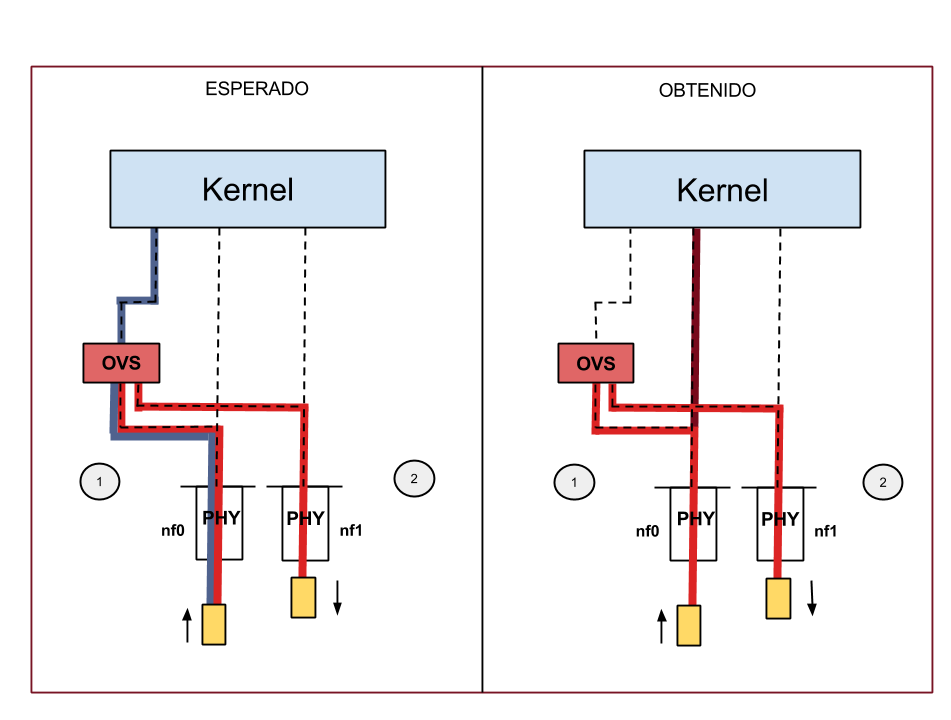
\includegraphics[width=0.75\textwidth]{ovs_figure3}
\caption[OVSInterfaces]{Descripci\'on esquematica de interfaces propuesta}
\label{fig:OVSInterfaces}
\end{figure}


\newpage
\begin{figure}[htbp!] 
\centering    
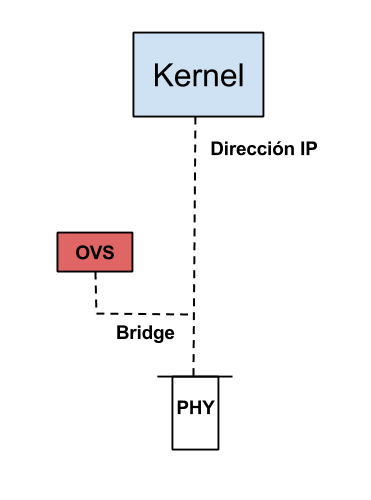
\includegraphics[width=0.3\textwidth]{ovs_figure1}
\caption[OVSInterfaces1]{Descripci\'on esquematica de interfaces en ovs}
\label{fig:OVSInterfaces1}
\end{figure}

\begin{figure}[htbp!] 
\centering    
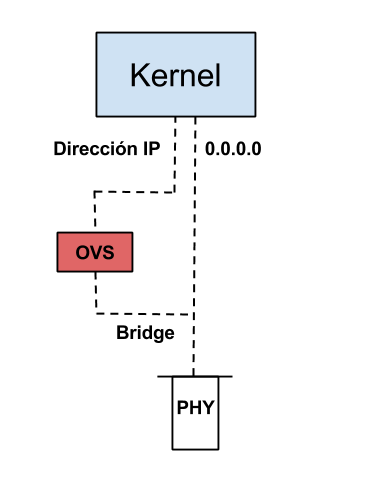
\includegraphics[width=0.3\textwidth]{ovs_figure2}
\caption[OVSInterfaces2]{Descripci\'on esquematica de interfaces propuesta}
\label{fig:OVSInterfaces2}
\end{figure}


Originalmente, para constru\'ir una interfaz IP con un puerto OpenFlow 

\begin{itemize}
\item Como se esperaria que se cmportara
\item Como se esta comportando
\item Porque se comporta asi
\item Como lo solucionamos
\end{itemize}

\end{enumerate}

\section{MPLS Linux y Quagga LDP}
Bueno creo que es aca donde sacarnos las ganas de hablar de Quagga LDP y MPLS linux

Que es MPLS LINUX, las dos versiones que hay, que es quagga LDP las dos versiones que hay.

Con que se empezo, que problemas tuvimos. Poca documentacion o practicamente nada.

Se recompila kernel, cambia configuracion, se logra configuracion intermedia.

La version original de MPLS Linux, no andaba porque no soportaba openvswitch, no reconocia la placa etc.

Ademas no compilaba la version que estaba en repositorio. Tenia errores de compilacion, faltaban herramientas para instalar que no existian. Muchos pero muchos problemas tecnicos.

Se probaron kernels desde la 3.09.algo hasra la 3.11.26 creo generic, a unas versiones mas viejas. En la confuguracion del kernel no estaba disponible MPLS, Openvswitch, un asco todo.

Se logor hacer andar el MPLS linux nuevo con el LDP nuevo.

Se podian insertar cosas en las tablas de MPLS y el quagga por si solo andaba. No obstante no funcionaba que se insertaran desde el LDP cosas a las tablas MPLS. En particular se moria cuando intentaba insertar la primer entrada de MPLS asociada a la tabla FTN para una fec en particualr. Debugueamos el codigo, inspeccionamos y acorralamos el bug pero no pudimos solucionarlo. Se co nsidero una perdida de tiempo asi que se siguio.

[make menuconfig]

\section{Instalaci\'on de Sistema Operativo}
Instalamos Fedora 14 y no booteaba. Desactivamos el uefi de la bios y tampoco. Probamos con varias versiones de Fedora incluso con un dvd de la uri y descargada de internet. Probamos con dvd y usb.

Fedeora 20 era compatible con la mother pero no encontrabamos driver para el cable programador.

Logramos instalar Xilinx en window XP SP3 con los drivers del cable. Aqui se podian programar las placas para las pruebas de aceptacion.

Probamos con Ubuntu 14.04, y las placas se reconocian el driver existia pero las pruebas de aceptacion no encaraban (fallaban todas). Problemas con el DMA.

Se probo con Ubuntu 12.04 y se logro instalar Xilinx, conseguir driver, reconocer placa y las pruebas de aceptacion ok!. 